\section{Durchführung}
In diesem Versuch wird die Schaltung aus Abbildung \ref{fig:schaltung} verwendet.
\begin{figure}[h]
    \centering
    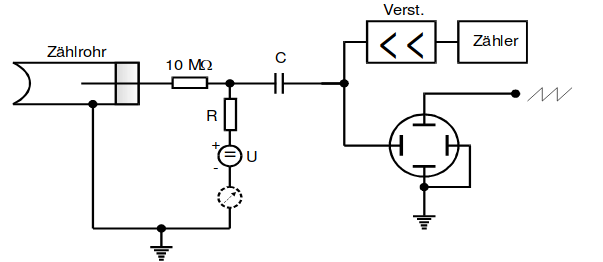
\includegraphics[height=4cm]{Aufbau/Schaltung.png}
    \caption{Prinzipieller Aufbau der Messapparatur.}
    \label{fig:schaltung}
\end{figure}
Im ersten Versuchsteil wird eine $\beta$-Quelle untersucht, indem sie vor das das Eintrittsfenster des Zählrohrs gestellt wird.
Dann werden 40 Messwerte im Bereich 300-700V aufgenommen, wobei die Spannung nicht über 700 V gewählt werden darf um das Zählrohr nicht zu zerstören.
Außerdem werden immer Messungen von 60s gemacht.\\
Im zweiten Versuchsteil wird die Totzeit auf zwei Wegen bestimmt.
Der erste Weg erfolgt über einfache Ablesung auf dem Oszilloskop.
Der zweite Weg erfolgt über die Messung zweier Proben.
Zunächst wird die Impulsrate der ersten Probe gemessen, daraufhin die Impulsrate beider Proben zusammen und zuletzt die Impulsrate der zweiten Probe.
Dabei ist es wichtig, diese Reihenfolge einzuhalten um die Lage der ersten Probe und danach die Lage der zweiten Probe relativ zum Eintrittsfenster nicht zu verändern.
